\documentclass{report}
\usepackage[backend=biber,style=numeric]{biblatex}
\addbibresource{references.bib}
\usepackage{graphicx} % Required for inserting images
\usepackage{subcaption}
\usepackage{booktabs} % For better table formatting
\usepackage{float}
\usepackage{hyperref} % Include the hyperref package for creating hyperlinks


\begin{document}
\begin{titlepage}
    \centerline{\Huge\textbf{GreenAI Documentation}}
    
    \vspace*{1cm}
    
    \centerline{
\includegraphics[width=16cm]{thws_logo.png}}
    
    \vspace*{1.5cm}
    
    \centerline{\LARGE Würzburg, Germany}
    
    \vspace*{1cm}
    
    \centerline{\Large{Illia Rohalskyi}}
    \vspace{0.2cm}
    \centerline{\large\textit{Matriculation Number: 9123047}}



    \vspace*{0.5cm}
    
    \centerline{\Large{Oskar Herkt}}
    \vspace{0.2cm}
    \centerline{\large\textit{Matriculation Number: 5021064}}
    
    \vspace*{1cm}
    
    \centerline{\LARGE{Supervised by Frank-Michael Schleif}}
    
        
\end{titlepage}

\tableofcontents

\chapter{Introduction}

\section{Project Overview}

The rapid advancement of artificial intelligence (AI) has spurred a remarkable rise in the complexity and resource demands of state-of-the-art models. A recent study conducted by researchers at the University of Massachusetts highlighted the significant environmental impact of training large AI models. The study revealed that training these models can produce approximately 626,000 pounds of carbon dioxide, equivalent to around 300 round-trip flights between New York and San Francisco—nearly five times the lifetime emissions of the average car \cite{strubell2019}. This stark contrast underscores the urgent need for a paradigm shift in how we approach AI research and deployment.

As highlighted by Strubell et al.~\cite{strubell2019}, the carbon footprint of training AI models has become a critical concern. Their landmark study demonstrated the substantial environmental impact associated with the development and deployment of sophisticated AI systems, revealing an urgent need for a more sustainable approach to AI research and deployment.

This realization has catalyzed a broader conversation within the AI community. Schwartz introduced the concept of Green AI, defining it as “AI research that yields novel results while taking into account the computational cost” \cite{schwartz2020}.

Despite these insights, achieving Green AI presents significant challenges. The complexity of AI systems necessitates a holistic approach that addresses all stages of their lifecycle—from data collection and model training to monitoring and deployment \cite{haakman2021}. Moreover, the field’s heterogeneity complicates efforts to obtain a comprehensive understanding of existing research and practices.

To address these gaps, our GreenAI project offers a solution that integrates strategic planning, cost estimation, and optimization for AI model training. By providing detailed analyses of financial and environmental impacts, and offering intelligent recommendations for balancing these factors, GreenAI aims to guide organizations toward more sustainable AI practices. This approach not only aligns with the growing emphasis on Green AI but also addresses the practical challenges faced by businesses in reducing the carbon footprint of their AI operations.

The growing maturity of the Green AI field underscores the necessity for increased industry engagement. Our project is designed to facilitate this transition, ensuring that AI advancements can be pursued without compromising environmental sustainability.

\begin{figure}[h!]
    \centering
    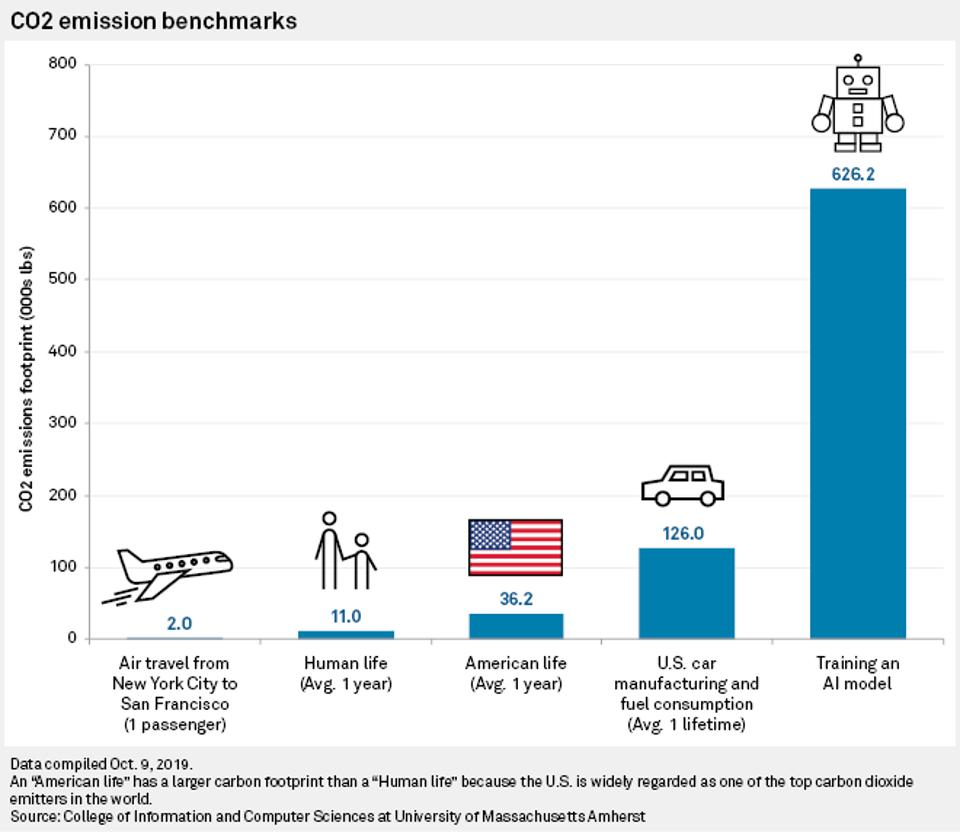
\includegraphics[width=\textwidth]{1.png}
    \caption{The contrast between the carbon footprint produced by training an AI model and the average lifetime emissions of people and automobiles. Image: spglobal.com}
    \label{fig:carbon_footprint}
\end{figure}

\section{Target Audience}

The GreenAI project is designed to address the needs of various stakeholders involved in the development and deployment of AI systems. Our target audience includes:

1. \textbf{Project Managers:} These individuals are responsible for overseeing AI projects and ensuring that they remain within budget and on schedule. They face the challenge of managing the increasing complexity and resource demands of AI models while also considering environmental impacts. GreenAI provides project managers with tools for strategic planning and cost estimation, enabling them to make informed decisions that align with sustainability goals.

2. \textbf{Business Leaders:} Executives and decision-makers who need to align AI initiatives with broader corporate sustainability objectives. As pressure to address environmental concerns grows, GreenAI offers business leaders insights into the financial and ecological impacts of their AI models. By incorporating GreenAI’s recommendations, they can ensure that their AI strategies drive innovation while contributing to their organization’s commitment to environmental stewardship.

3. \textbf{Sustainability Officers:} These professionals are focused on integrating sustainable practices into business operations. GreenAI provides them with essential data and recommendations to evaluate and improve the environmental impact of AI technologies, supporting their efforts to meet sustainability targets and enhance their organization's green credentials.

4. \textbf{Academic Researchers and Industry Analysts:} Individuals studying the intersection of AI and sustainability will find GreenAI’s insights valuable for their research. The project contributes to the growing body of work aimed at advancing Green AI practices by offering detailed analyses and recommendations that can inform future studies and industry practices.

In summary, GreenAI serves a diverse audience of professionals committed to advancing AI technologies while addressing critical issues of environmental sustainability. The project equips them with the tools and knowledge necessary to navigate the complexities of AI model training and deployment, ensuring that their efforts contribute positively to both technological innovation and ecological preservation.



\section{Problem Statement}

The exponential growth of AI has led to a dramatic increase in the resources required for training models. This surge in demand is reflected in the growing need for high-performance computing resources, such as GPUs, and the associated rise in energy consumption. These factors contribute to higher operational costs and an escalating environmental impact, with a notable increase in the carbon footprint due to the energy-intensive nature of AI training.

In the quest for technological advancement, these challenges are often overlooked. However, as organizations scale their AI operations, the financial and environmental implications become increasingly critical. GreenAI addresses this problem by offering clear, data-driven estimates of the financial and environmental costs associated with AI training. It also helps organizations optimize their training strategies to balance sustainability with costs and time, ultimately enabling more sustainable and cost-effective AI innovation.

\chapter{Getting Started}


The first step in using the GreenAI application is to clearly define the task or problem you aim to solve. For instance, you might want to create a model that detects cars in images. Accurately defining your task is crucial as it directly influences the system's recommendations regarding hardware selection, model architecture, and training strategy.

Next, you need to provide details about the dataset that will be used to train the model. For example, you might specify a dataset containing 1 million images of cars with bounding boxes. The dataset size and type are essential factors because they determine the computational resources required and affect the model's performance.

After setting up the task and dataset, you will need to provide the following key inputs:

\begin{itemize}
    \item \textbf{Performance Needs}: This defines how precise or efficient your model should be. For instance, tasks such as medical diagnostics or real-time object detection demand high precision. On the other hand, if performance flexibility is acceptable, you can indicate that in your input.
    \item \textbf{Time}: Specify the amount of time available for training the model. Training deep learning models can range from hours to days or even weeks depending on their complexity. Defining how quickly you need the results is important for planning.
    \item \textbf{Budget}: Training AI models, especially on high-performance GPUs, can be costly. To ensure the system suggests hardware options that match your financial constraints, you should clearly outline your budget.
    \item \textbf{Eco-Friendliness}: If minimizing carbon emissions is a priority for your project, you can indicate that. Alternatively, if eco-friendliness is not a major concern, you can select "Not Important" for this parameter.
\end{itemize}

In addition to these key inputs, GreenAI offers optional fields to give you even more control over the process:

\begin{itemize}
    \item \textbf{Maximum Time}: This allows you to set an upper limit on how long the training process can take.
    \item \textbf{Maximum Cost}: You can define the maximum amount you are willing to spend on training your model.
    \item \textbf{Maximum CO2 Emissions}: If environmental impact is a concern, you can set a limit on the allowable CO2 emissions (in kg) for the training process.
\end{itemize}

If you choose to leave any of these optional fields blank, the system will automatically use default values to keep the process going smoothly. By default, there will be no limits on cost or CO2 emissions, and the available time will be considered unlimited.

Once all the required fields have been filled out, you can submit the form. The system will process the provided information and, after a brief moment, will generate a Project Overview. This overview will include:

\begin{itemize}
    \item The weightings assigned to eco-friendliness, cost, and time based on your inputs.
    \item A recommendation for the best model architecture for your task.
    \item A suggested training strategy.
    \item An explanation of why the chosen architecture and strategy were recommended based on the inputs you provided.
\end{itemize}
\begin{figure}[!h]
    \centering
    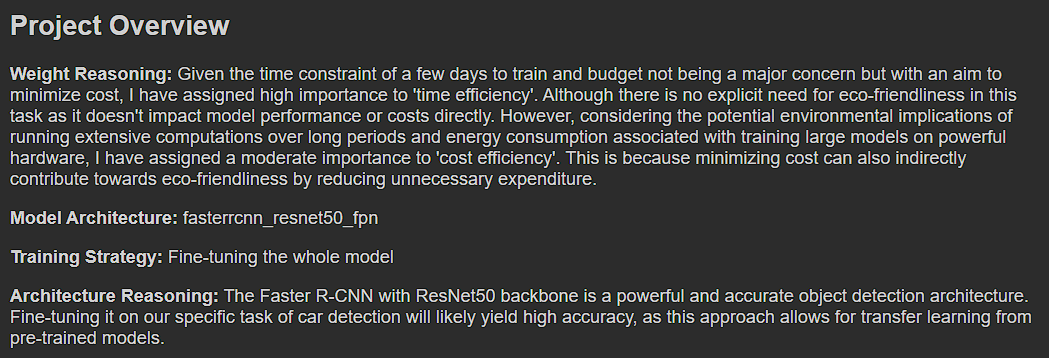
\includegraphics[width=1\linewidth]{PORichitg.png}
    \caption{Project Overview showing  User the Reasoning of the AI.}
    \label{fig:enter-label}
\end{figure}

\newpage
Following the Project Overview, you receive a detailed \textbf{Results Table}, which ranks GPUs based on their Overall Score wich has been weighted for your task. The key metrics displayed in the table include:

\begin{itemize}
    \item \textbf{CO2 (kg)}: The estimated carbon emissions associated with training the mode.
    
    \item \textbf{Cost (\$)}: The estimated cost for using the GPU during model training.
    
    \item \textbf{Region}: The geographical location of the GPU, which could impact availability.
    
    \item \textbf{Time}: The estimated time required to complete model training on one GPU.
    
    \item \textbf{CO2 Score}: A 5-star rating that shows the environmental impact of each GPU.
    
    \item \textbf{Time Score}: A star rating that shows how quickly the GPU can complete the task.
    
    \item \textbf{Cost Score}: A star rating that shows how cost-efficient each GPU is.
    
    \item \textbf{Overall Score}: A composite star rating that represents the overall suitability of the GPU, factoring in performance, cost, time, and eco-friendliness, based on the User's preference.
\end{itemize}

\begin{figure}[h]
    \centering
    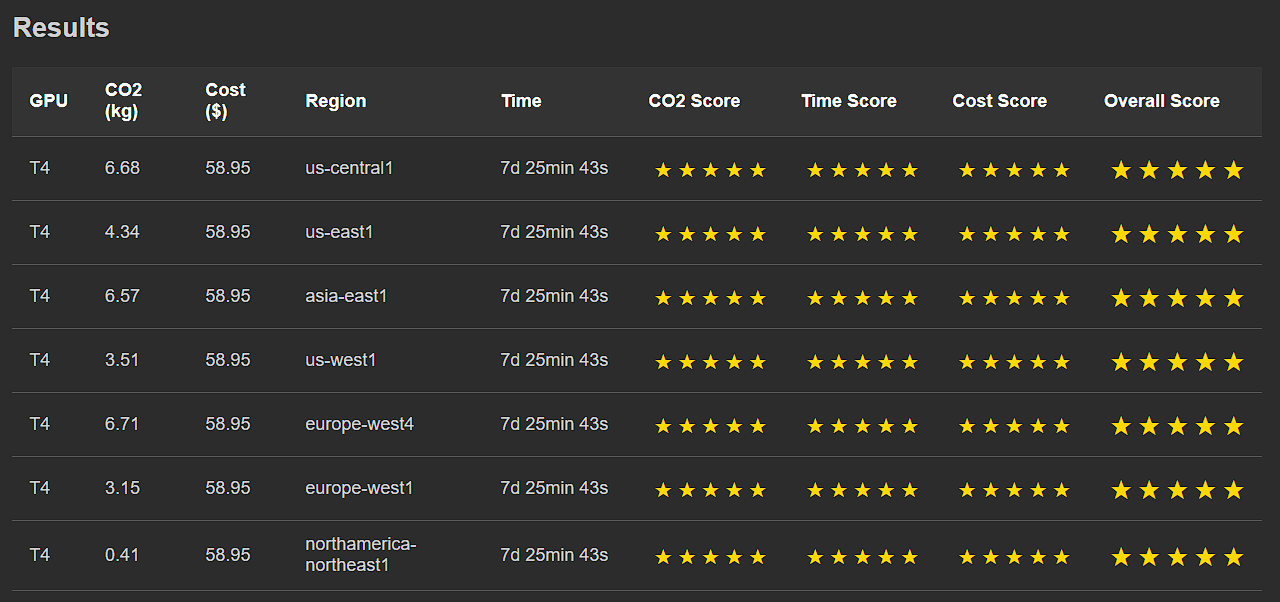
\includegraphics[width=1\linewidth]{04.png}
    \caption{Result Table with Star Rating for easy Overview.}
    \label{fig:enter-label}
\end{figure}

Each of these scores is displayed as a star rating, with additional functionality that allows you to hover over the stars to see the exact score to two decimal places. The \textbf{Overall Score} is displayed with larger stars to emphasize its importance in making the final decision.

By providing these features and metrics, GreenAI offers a comprehensive and customizable platform for optimizing hardware recommendations based on the specific needs of your machine learning task.



\chapter{User Interface Overview}

The GreenAI interface is designed to be user-friendly and intuitive, while still offering detailed control over input and output options. The layout allows users to seamlessly define their task, set constraints, and view the results.

\section{Input Fields}
At the top of the interface, users can define their machine learning task, specify the dataset, and describe the performance needs. The following key input fields are provided:

\begin{itemize}
    \item \textbf{Task}: A description of the problem the user is trying to solve (e.g., "build a model to detect cars in images").
    \item \textbf{Dataset}: Information about the data available for training the model (e.g., "1 million images of cars with bounding boxes").
    \item \textbf{Performance Needs}: How precise or efficient the model should be.
    \item \textbf{Time}: How much time is available to train the model.
    \item \textbf{Budget}: The financial constraints for training the model.
    \item \textbf{Eco-Friendliness}: The importance of minimizing the environmental impact during training.
    \item \textbf{Maximum Time, Maximum Cost, Maximum CO2}: Optional fields allowing users to set upper limits on time, cost, and carbon emissions.
\end{itemize}

Each input field comes with an optional \textbf{“Not Important”} checkbox, which allows users to deprioritize specific aspects of their project, offering flexibility when configuring the system. Mandatory Inputs include: Task, Dataset. Not making any Inputs will give the User a warning telling the User to add the Input.
\begin{figure}
    \centering
    
\includegraphics[width=0.5\linewidth]{warning.png}
    \caption{Warning for missing inputs}
    \label{fig:enter-label}
\end{figure}

\section{Submit Button}
Once all input fields are filled out, the user can press the \textbf{Submit Button} to process their request. The system then sends the data to the Backend, which processes the information and provides results. After a brief period, typically under a minute (depending on the graphics card), the system returns the optimized recommendations based on the user’s inputs.

\section{Tooltips}
To enhance user experience, the interface includes \textbf{tooltips} that appear when hovering over the star ratings. These tooltips display the exact values (rounded to two decimal places) for CO2, Time, Cost, and Overall Scores. This feature allows users to get a detailed breakdown of each score before making their selection.

\section{User Experience and Navigation}
The interface is designed to cater to both technical and non-technical users:

\begin{itemize}
    \item The input section provides a clear and concise way to define tasks and constraints.
    \item The results section offers an easy-to-navigate comparison of GPUs, with star ratings simplifying decision-making.
    \item The use of tooltips and visual elements such as stars ensures that even complex metrics like environmental impact and cost-efficiency are communicated in an understandable manner.
\end{itemize}

So using the GreenAI interface strikes a balance between simplicity and advanced functionality, providing a seamless workflow from task definition to GPU selection based on time, cost, and eco-friendliness considerations.


\chapter{System Architecture and Data Flow}

\begin{figure}[h]
    \centering
    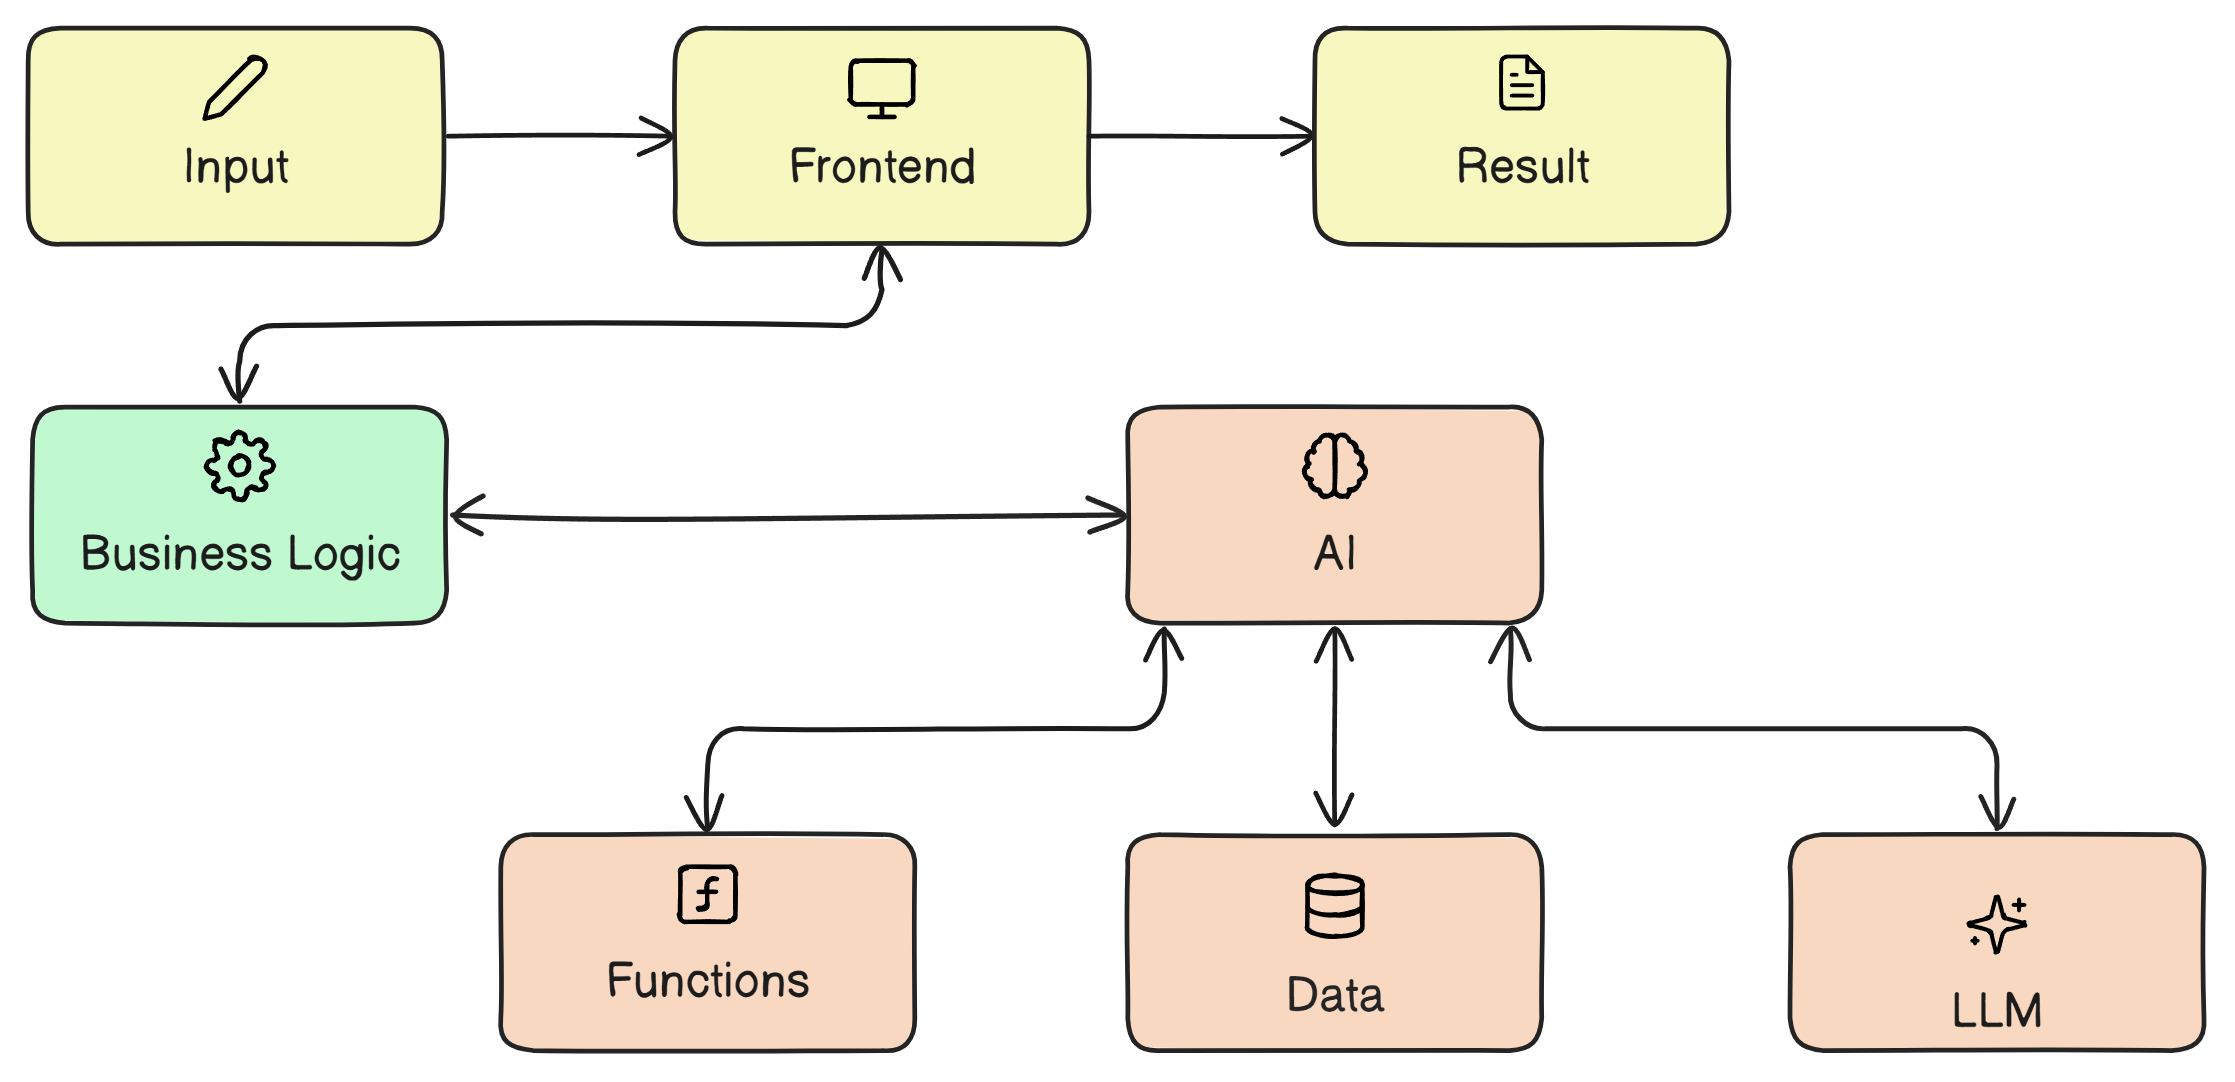
\includegraphics[width=1\linewidth]{Archfertig.png}
    \caption{ystem Architecture Diagram showing the interaction between the Input, Frontend, Business Logic, and AI components in GreenAI.}
    \label{fig:enter-label}
\end{figure}

The architecture of the GreenAI system is structured to manage user inputs, process the data, and deliver optimized hardware and training recommendations. The system consists of several key components: \textbf{Input}, \textbf{Frontend}, \textbf{Business Logic}, \textbf{AI} (with subcomponents \textit{Functions}, \textit{Data}, and \textit{LLM}), and the \textbf{Result}. Each component plays a critical role in ensuring the efficiency and effectiveness of the system. Below is a detailed breakdown of how these components interact and the flow of data between them.

\section{Input}
The \textbf{Input} component is the first point of interaction where users provide the essential details for the project. It allows users to define the task, dataset, and constraints like performance, time, budget, and eco-friendliness. Additionally, users can input upper limits for time, cost, and CO2 emissions, giving them fine-grained control over resource allocation.

\begin{itemize}
    \item \textbf{User Input}: Users fill out fields such as task description, dataset size, performance needs, and optional fields for maximum time, cost, and CO2 emissions.
    \item \textbf{Form Submission}: After completing the form, the submission triggers a request that sends all user inputs to the backend via a HTTP POST request, initiating the next phase of processing in the system.
\end{itemize}

\section{Frontend (User Interface)}
The \textbf{Frontend} or \textbf{User Interface} handles the visual and interactive aspects of the system. It captures user inputs and presents the results, including detailed comparisons of hardware options. The interface is designed to be intuitive and allows for easy navigation through various input fields and result sections.

\begin{itemize}
    \item \textbf{Data Capture}: The user interface captures input fields such as task, dataset, performance requirements, and constraints (time, budget, and eco-friendliness).
    \item \textbf{Display of Results}: Once the Business Logic and AI components complete their calculations, the frontend displays the recommendations in a structured table with metrics and star ratings.
\end{itemize}

\section{Business Logic}
The \textbf{Business Logic} is the middleware that processes the user inputs, validates them, and passes them to the AI layer for further computation. It ensures that data flows smoothly between the frontend and the AI component.

\begin{itemize}
    \item \textbf{Input Validation}: Validates the user inputs, checking for completeness and correctness, while applying default values where necessary.
    \item \textbf{State Creation}: After validation, a \texttt{MainState} object is created, encapsulating the user's input. This includes optional values like maximum time, cost, and CO2.
    \item \textbf{Forwarding to AI}: Once the data is structured, the Business Logic forwards the validated inputs to the AI component for heavy computational tasks like model generation and ranking.
\end{itemize}

\section{AI }
The \textbf{AI} layer performs the core computations. It handles data retrieval, applies machine learning models, and generates rankings based on the user’s constraints and inputs.

\begin{itemize}
    \item \textbf{Functions}: The AI runs machine learning models and functions to compute the best hardware recommendations based on the dataset and task.
    \item \textbf{Data}: The system retrieves GPU data, including performance metrics, cost, time efficiency, and CO2 emissions. This data is critical for generating accurate recommendations.
    \item \textbf{LLM (Large Language Model)}: The LLM is used for generating, refining, and optimizing recommendations. It selects the most appropriate machine learning models (e.g., ResNet-18) and training strategies (e.g., Last Layer Learning) based on the user’s time, budget, and performance constraints.
\end{itemize}

\subsection{Grading}
The AI system calculates scores based on the user's constraints:
\begin{itemize}
    \item \textbf{Time Efficiency}: Focuses on selecting faster GPUs for tasks with tight time constraints.
    \item \textbf{Cost Efficiency}: Recommends budget-friendly GPUs when cost is a priority.
    \item \textbf{Eco-friendliness}: Suggests GPUs with lower CO2 emissions when environmental impact is prioritized.
\end{itemize}

\subsection{Ranking and Scoring}
The AI ranks the available GPUs based on multiple factors:
\begin{itemize}
    \item \textbf{CO2 Score}, \textbf{Time Score}, \textbf{Cost Score}: Each GPU is evaluated and rated based on these metrics, with star ratings visualized in the user interface.
    \item \textbf{Overall Score}: A composite score based on all the factors is also displayed, providing an overarching recommendation for each GPU.
\end{itemize}

\section{Result}
The \textbf{Result} component presents the outcome of the system’s processing. It shows the final recommendations for GPUs and other hardware in a table, highlighting key metrics like CO2 emissions, time, and cost.

\begin{itemize}
    \item \textbf{Ranking}: Each GPU is ranked according to its suitability for the task.
    \item \textbf{Star Ratings}: Metrics such as CO2, Time, and Cost are visually represented using star ratings, with detailed values available via tooltips.
\end{itemize}

\section{Data Flow}
The following outlines the flow of data through the system:

\begin{itemize}
    \item \textbf{Input to Frontend}: Users enter their project requirements in the Input section, which is handled by the Frontend component.
    \item \textbf{Frontend to Business Logic}: Once the form is submitted, the data is sent from the Frontend to the Business Logic for validation and structuring.
    \item \textbf{Business Logic to AI}: After validation, the Business Logic forwards the inputs to the AI, where data is retrieved, models are generated, and hardware is ranked.
    \item \textbf{AI Processing}: The AI layer retrieves GPU data, generates recommendations using models and strategies, and calculates rankings based on user constraints (time, cost, CO2).
    \item \textbf{AI to Business Logic}: The results, including ranked GPUs and star ratings, are passed back to the Business Logic.
    \item \textbf{Business Logic to Frontend}: Finally, the Business Logic sends the processed results to the Frontend, where they are displayed to the user in a structured format.
\end{itemize}

This flow ensures that user inputs are efficiently processed and optimized hardware recommendations are generated and presented in a user-friendly manner.


\chapter{The Intelligence Behind GreenAI}

In this chapter, we delve into the core mechanisms of GreenAI, focusing on how nodes and edges in the \texttt{langgraph} framework drive our decision-making processes. This system is structured to optimize the eco-friendliness, time efficiency, and cost efficiency of AI training tasks, balancing complex trade-offs across performance, energy consumption, and financial constraints.

\section{High-Level Overview}

GreenAI operates as a decision-making engine that recommends the most suitable model architecture, training strategy, and computational resources for a given task. It processes input data such as the model type, task specifications, and constraints, then ranks various GPU configurations based on their trade-offs. 

The workflow is modeled using \texttt{langgraph}'s \texttt{StateGraph}, which allows for cycles and stateful operations:

\begin{itemize}
    \item \textbf{Nodes} represent distinct decision points, such as priority ranking, architecture recommendations, and resource cost calculations.
    \item \textbf{Edges} represent the transitions between decision points, including conditional edges that allow for iterative refinement of recommendations.
\end{itemize}

\section{Input and Output}

\subsection{Input}
The system receives a set of parameters to guide its recommendations and decision-making process. The input includes the following \textbf{soft constraints}:

\begin{itemize}
    \item \textbf{Task Description:} A clear statement of the objective or goal for the model or system being configured.
    \item \textbf{Data Description:} Details about the dataset, including its size, format, and any preprocessing steps that have been applied.
    \item \textbf{Performance Needs:} The desired level of performance or accuracy that the model should achieve.
    \item \textbf{Time Constraint:} The rough time frame within which the model or system should be completed or operational.
    \item \textbf{Budget Constraint:} Any financial limitations or considerations that affect the cost of the solution.
    \item \textbf{Eco-Friendliness:} Any requirements related to the environmental impact of the model or system.
\end{itemize}

Additionally, the input may include \textbf{hard constraints}:
\begin{itemize}
    \item \textbf{Maximum Time:} The absolute maximum amount of time in seconds allowed for the process or model training, which must not be exceeded.
    \item \textbf{Maximum Cost:} The absolute financial limit that should not be surpassed.
    \item \textbf{Maximum CO2 Emissions:} The maximum allowable carbon footprint, which is strictly enforced.
\end{itemize}

\textbf{Hard Constraints vs. Soft Constraints:}
\begin{itemize}
    \item \textbf{Hard Constraints:} These are non-negotiable limits that must be strictly adhered to. The system cannot exceed these constraints under any circumstances.
    \item \textbf{Soft Constraints:} These are preferences or goals that guide the system’s recommendations but are not strictly enforced. The system aims to meet these requirements as closely as possible, within the boundaries set by the hard constraints.
\end{itemize}


\subsection{Output}
The system produces results based on the input parameters, which typically include:

\begin{itemize}
    \item \textbf{Recommended Solution:} A detailed suggestion for the configuration or approach that best fits the specified task and constraints.
    \item \textbf{Strategy:} An optimal plan or method for achieving the desired performance within the given constraints.
    \item \textbf{Estimates:} Estimated values for key factors such as time, cost, and environmental impact.
    \item \textbf{Rankings and Recommendations:} A ranked list of options or configurations based on their alignment with the input parameters and constraints.
\end{itemize}

\section{Data Sources}

GreenAI utilizes several data sources:

\begin{itemize}
    \item \texttt{model\_flops.xlsx}: Contains information about various AI models and their Floating Point Operations (FLOP) requirements.
    \item \texttt{GCP gpus pricing.xlsx}: Provides pricing information for different GPU configurations on Google Cloud Platform.
    \item \texttt{gpus.csv}: Contains performance data for various GPUs, including Tera Floating Point Operations Per Second (TFLOPS) and Thermal Design Power (TDP).
    \item \texttt{impact.csv}: Provides region-specific carbon intensity data for emissions calculations.
\end{itemize}

\noindent The data for \texttt{gpus.csv} and \texttt{impact.csv} can be found at the following GitHub repository: \\
\url{https://github.com/mlco2/impact/tree/master/data}


\section{Language Model}

GreenAI uses the Ollama framework with the Phi3 Mini model for natural language processing tasks. The model is configured with the following parameters:

\begin{itemize}
    \item Model: phi3:mini
    \item Temperature: 0
    \item Top-p: 0.2
    \item Format: JSON
\end{itemize}

Empirical results show that this model with the specified parameters offers optimal performance without compromising time or computational efficiency.
\section{How the Nodes and Edges Work Together}

GreenAI's core flow is structured around three main stages:

\subsection{Priority Assignment (ranking\_node)}
\textbf{Input:} MainState object containing task description, data info, performance needs, time and budget constraints, and eco-friendliness preferences.

\vspace{0.2cm}

\textbf{Process:}
\begin{enumerate}
    \item Constructs system and human messages using the input state.
    \item Invokes the Phi3 Mini model.
    \item Normalizes the returned weights to sum to 1.0.
\end{enumerate}

\textbf{Output:} Updated MainState with normalized \texttt{eco\_weight}, \texttt{time\_weight}, \texttt{cost\_weight}, and \texttt{weight\_reasoning}.

\subsection{Architecture Recommendation (architecture\_node)}
\textbf{Input:} MainState object with priority weights and task information.

\vspace{0.2cm}

\textbf{Process:}
\begin{enumerate}
    \item Selects appropriate prompt based on \texttt{simplification\_attempts}.
    \item Constructs messages with task info and priorities.
    \item Invokes the Phi3 Mini model.
\end{enumerate}

\textbf{Output:} Updated MainState with \texttt{model\_architecture}, \texttt{training\_strategy}, \texttt{tflops\_precision}, and \texttt{architecture\_reasoning}.

\subsection{GPU Configuration Calculation (calculator\_node)}
\textbf{Input:} MainState object with architecture recommendation and priority weights.

\vspace{0.2cm}

\textbf{Process:}
\begin{enumerate}
    \item Invokes model to estimate sample count, input size, and epochs.
    \item Calls \texttt{recommend\_gpu\_configuration()} function, which:
    \begin{itemize}
        \item Estimates total FLOPs using \texttt{estimate\_flops()}.
        \item Calculates training time for each GPU using \texttt{estimate\_time()}.
        \item Computes energy consumption with \texttt{calculate\_kwh\_consumption()}.
        \item Estimates CO2 emissions using \texttt{calculate\_emissions()}.
        \item Calculates cost with \texttt{calculate\_price()}.
    \end{itemize}
    \item Normalizes and scores results based on priority weights.
\end{enumerate}

\textbf{Output:} Updated MainState with \texttt{dataframe} containing ranked GPU configurations, updated \texttt{simplification\_attempts}, and \texttt{constraints\_met} flag.

After each node's execution, the updated MainState is passed to the next node or used to determine the next action via the conditional edge.
\section{Conditional Edge and Iterative Refinement}

A critical feature of GreenAI is its capability to refine recommendations when initial constraints are not met. This is achieved through the use of a conditional edge mechanism:

\begin{verbatim}
def should_simplify(state: MainState):
    return not state.constraints_met and state.simplification_attempts < 3

builder.add_conditional_edges(
    "calculator",
    should_simplify,
    {
        True: "architecturer",
        False: END
    }
)
\end{verbatim}

The conditional edge allows the system to revisit the architecture recommendation stage if the initial solution fails to meet all constraints. This is particularly important because the architecture node might initially propose a model and training strategy that are too resource-intensive to fit within the hard constraints, such as time or cost limitations. By cycling back to the architecture recommendation stage up to three times, the system can iteratively select a more feasible and lighter solution that adheres to all specified constraints. This iterative refinement process ensures that the recommendations are adjusted progressively until they satisfy the defined constraints, thereby optimizing the balance between performance, efficiency, and feasibility.

\section{State Management}

GreenAI uses a \texttt{MainState} class to manage the state throughout the decision-making process. This class includes fields for all relevant information, including:

\begin{itemize}
    \item Task and data descriptions
    \item Priority weights
    \item Current model architecture and training strategy recommendations
    \item Constraint information
    \item Number of simplification attempts
\end{itemize}

The state is passed between nodes and updated at each stage, ensuring that all decisions are made with full context.

\section{Graph Visualization}

To provide a visual representation of the GreenAI decision-making process, we include the final graph:

\begin{figure}[h!]
    \centering
    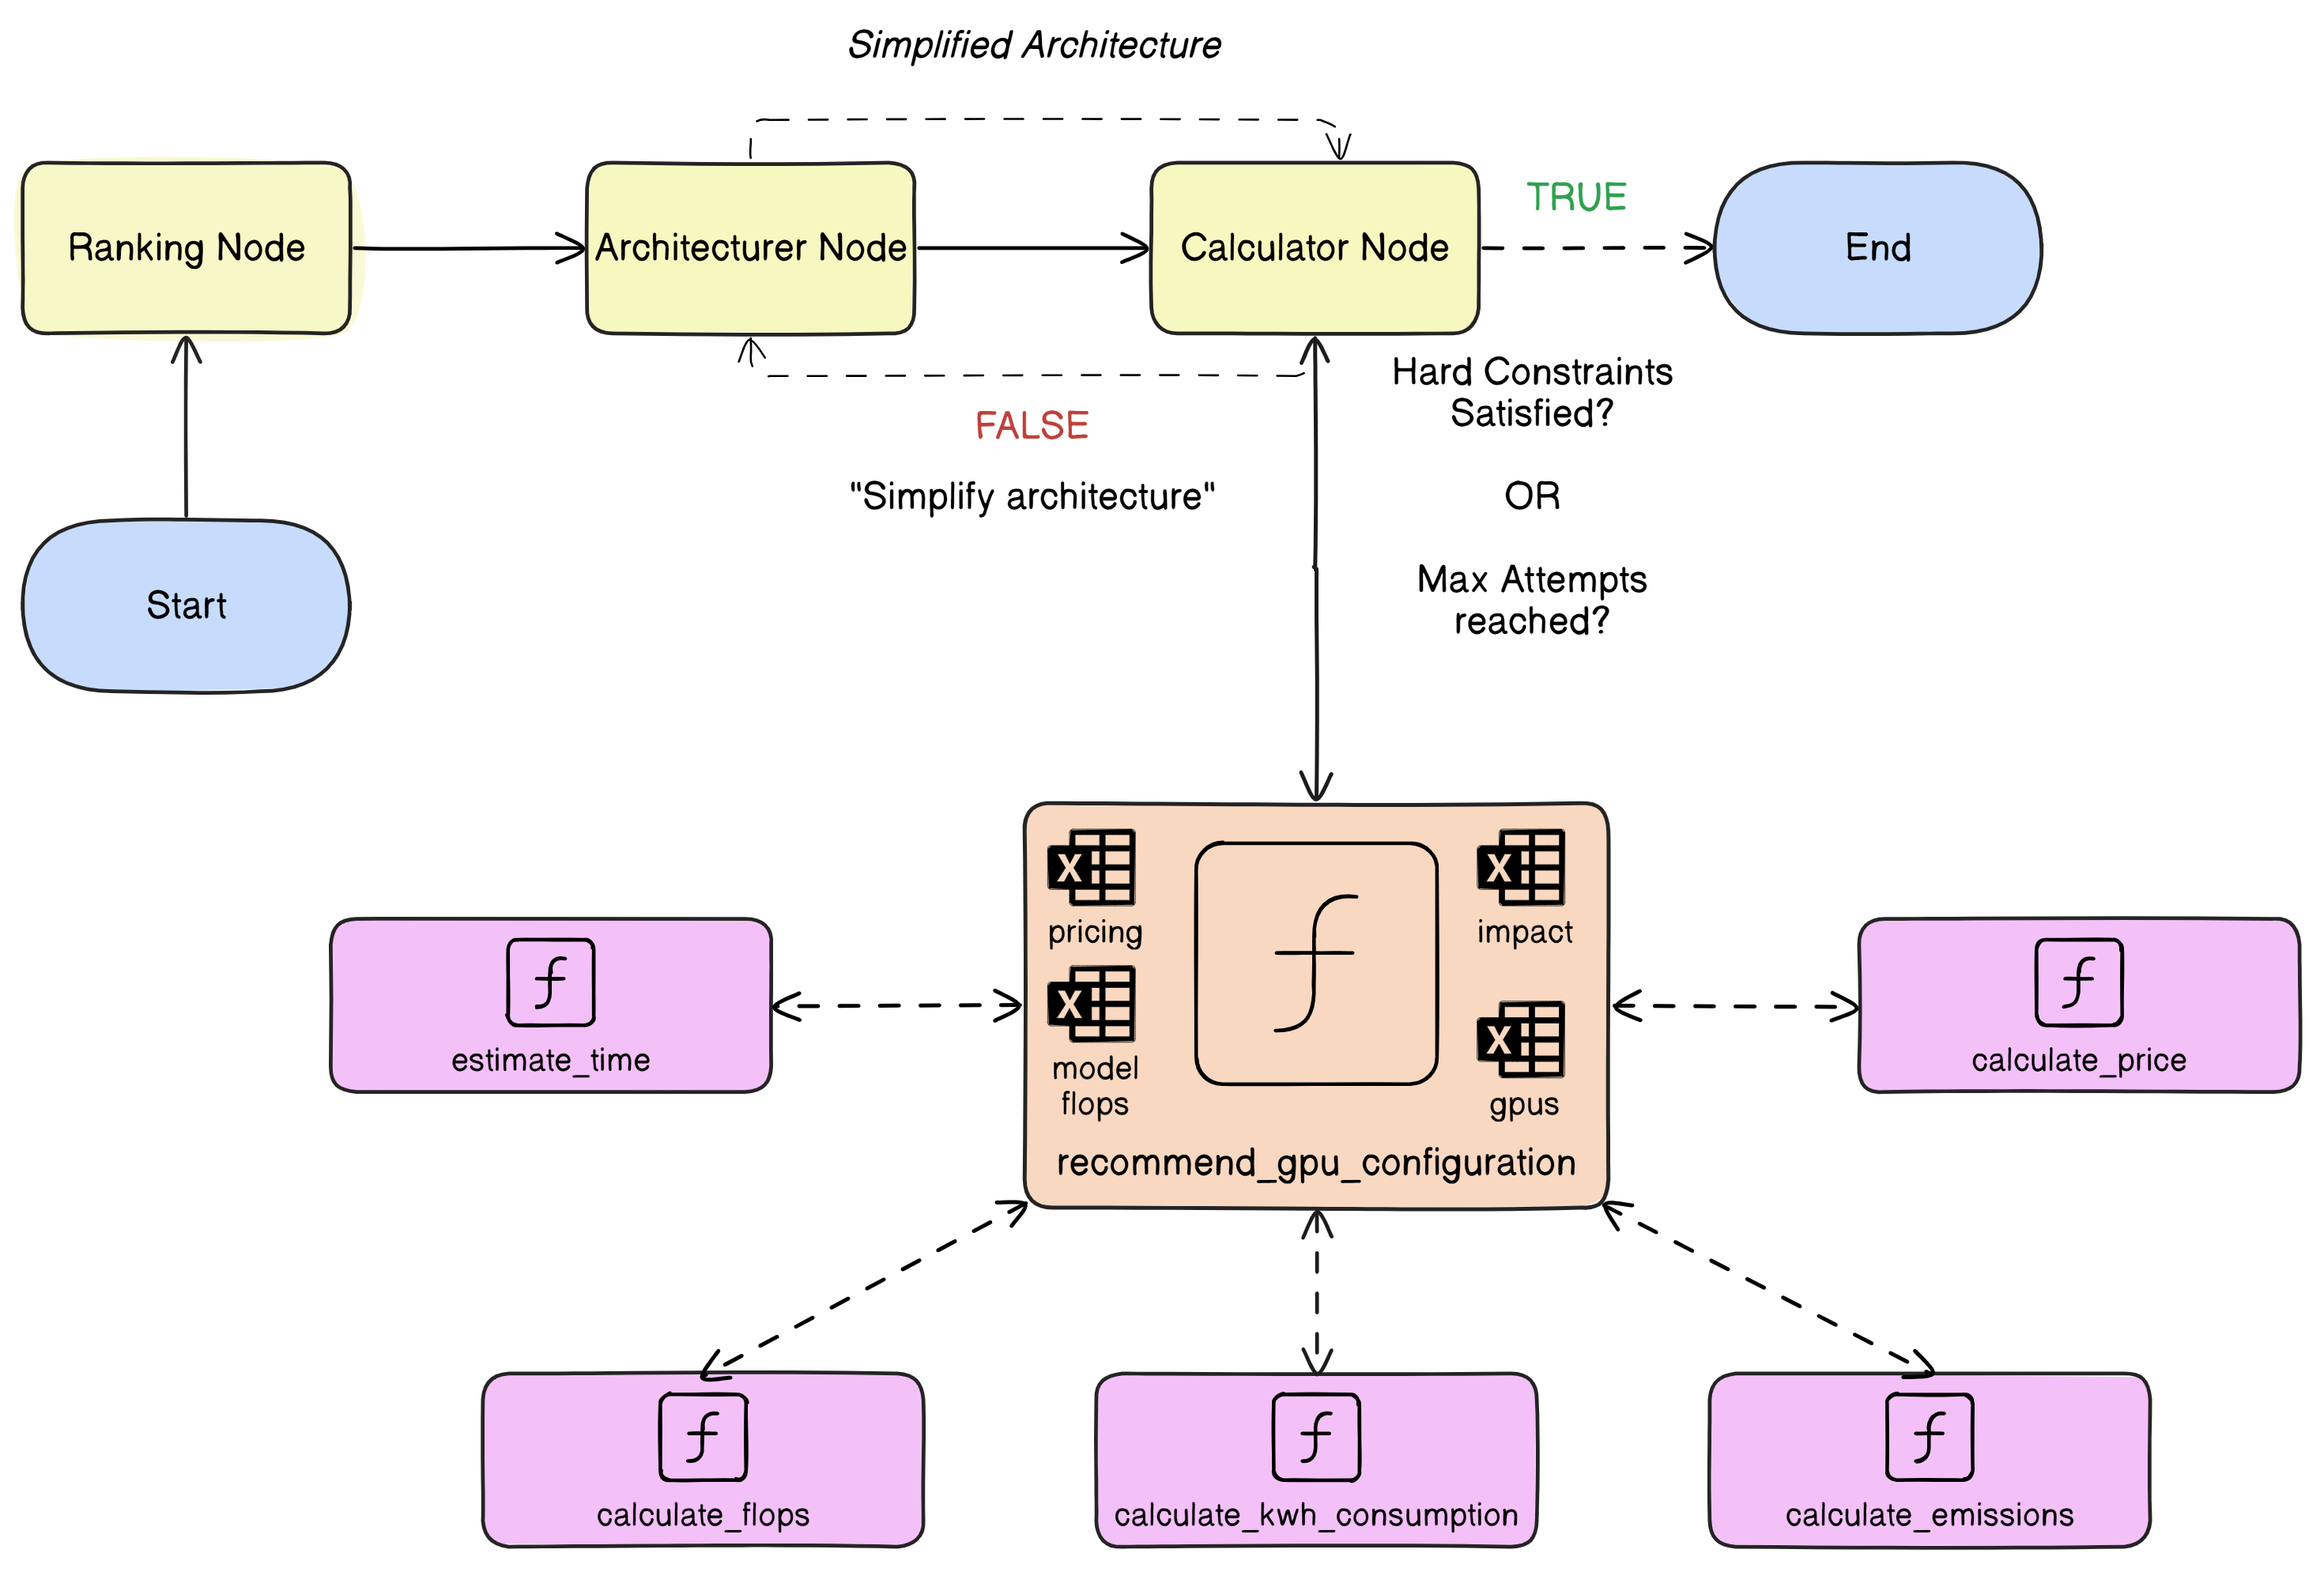
\includegraphics[width=\textwidth]{2.png}
    \caption{Final graph depicting the GreenAI decision-making process.}
    \label{fig:greenai_graph}
\end{figure}


\chapter{Case Studies}

GreenAI’s flexibility and range of options make it ideal for various use cases where Natural Language Processing or Computer Vision is used, each with different requirements for performance, cost, time, and eco-friendliness. This chapter outlines several case studies that demonstrate how GreenAI can be applied in different scenarios.


\section{Text Classification: Sentiment Analysis for Social Media}

A tech startup is building a text classification model to perform sentiment analysis on social media posts. The model will classify posts as positive, neutral, or negative. The company needs a balance between accuracy, quick processing, and eco-friendliness, while operating under a tight budget.

\begin{itemize}
    \item \textbf{Architecture Reasoning}: For this text classification task, the DistilBERT model is a strong choice. It offers a good balance between accuracy and computational efficiency, making it ideal for sentiment analysis. The model’s reduced size compared to the original BERT ensures faster training times, which is important for real-time processing.

    \item \textbf{Weight Reasoning}: The startup prioritizes cost efficiency (0.5) due to its limited budget, followed by time efficiency (0.3) as they require quick processing for real-time social media analysis. Eco-friendliness is also considered important (0.2) due to the company’s commitment to sustainability.

    \item \textbf{Model Architecture}: distilbert-base-uncased

    \item \textbf{Training Strategy}: Last Layer Learning
\end{itemize}



\section{Autonomous Vehicle}

A startup developing autonomous vehicle software needs to train models that can detect obstacles in real-time. The task requires extremely high accuracy due to the safety-critical nature of the application. The startup has relatively loose budget constraints but places a secondary focus on minimizing CO2 emissions where possible.

\begin{itemize}
    \item \textbf{Architecutre Reasoning}: Given the safety-critical nature of obstacle detection in autonomous vehicles, we prioritize accuracy. The 'Faster R-CNN ResNet50 FPN' model is a robust choice for object detection tasks and can be fine-tuned quickly due to its pre-trained weights on large datasets like COCO. 
    
    \item \textbf{Weight Reasoning}: Given the safety-critical nature of autonomous vehicle software and its requirement for extremely high accuracy within a short time frame, cost efficiency is prioritized to manage budget constraints effectively while still meeting performance needs. 
    
    \item \textbf{Model Architecture}: fasterrcnn\_resnet50\_fpn 
    
    \item \textbf{Training Strategy}:  Last Layer Learning 
\end{itemize}

\section{Image Processing in Low-Budget Startup}

A startup with limited funding is developing an image processing model for categorizing stock photography. They need a budget-conscious solution but can allow more time for training. Reducing costs is the top priority.

\begin{itemize}
    \item \textbf{Architecutre Reasoning}: Given the medium accuracy requirement and budget constraints, 'Last Layer Learning' is a cost-effective strategy that allows for fine-tuning on specific stock photography categories without extensive retraining. ResNet18 offers a balance between performance and computational efficiency. 
    
    \item \textbf{Weight Reasoning}: Given the startup's budget constraints and their willingness to allow more time for training without a strict deadline, cost efficiency is prioritized with a weight of 0.45. Time efficiency also holds importance due to its medium performance needs but receives slightly less priority at 0.3 because there are no immediate pressures on the project timeline that would necessitate rapid development and deployment. Eco-friendliness, while still considered important for corporate social responsibility reasons, is assigned a weight of only 0.25 as it's secondary to cost concerns in this scenario. 
    
    \item \textbf{Model Architecture}: resnet18 
    
    \item \textbf{Training Strategy}:  Last Layer Learning 
\end{itemize}

\chapter{Project Achievements and Future Improvements}

\section{Achievements}

\begin{itemize}
    \item \textbf{Fully Functional Hardware Recommendation System}: GreenAI successfully provides accurate hardware recommendations based on user-defined constraints. The system takes into account CO2 emissions, time, cost, and overall suitability, offering users environmentally friendly and cost-effective options for GPU usage.
    
    \item \textbf{Comprehensive Scoring and Ranking}: The platform’s multi-factor scoring system evaluates each GPU based on several dimensions:
    \begin{itemize}
        \item \textit{Eco-Friendliness (CO2 emissions)}: Provides a detailed rating system that helps users choose hardware with minimal environmental impact.
        \item \textit{Time Efficiency}: Recommends the fastest GPUs based on user-defined time constraints.
        \item \textit{Cost Efficiency}: Suggests the most budget-friendly GPUs when cost is prioritized.
    \end{itemize}
    The star-rating system with tooltips enhances user understanding of each GPU’s performance on these key metrics.

    \item \textbf{Flexible User Input}: GreenAI’s user interface allows for clear task specification, with options to define maximum limits for time, cost, and CO2 emissions. The flexibility to mark some factors as "Not Important" gives users control over how they want to prioritize their project’s performance, budget, or eco-friendliness.

    \item \textbf{Efficient Backend Processing}: The backend architecture integrates smoothly with the frontend and AI layers to process user input efficiently. It applies validation checks and prepares the input for computation from the AI.
\end{itemize}

\section{Future Improvements}

\begin{itemize}
    \item \textbf{Multi-GPU Support}: While the current system calculates values for individual GPUs, an important future enhancement would be the support for multi-GPU configurations. This would allow the system to recommend setups where multiple GPUs are used in parallel, optimizing training speed and performance.

    \item \textbf{Expanded GPU Database}: The system can be expanded to include a wider range of GPUs, ensuring that users have more options to choose from. By adding more GPUs to the database, the system would provide a broader selection of hardware, catering to different performance needs, budgets, and eco-friendliness preferences. 


    \item \textbf{Chatbot Integration}: A conversational chatbot could be integrated to guide users through the input process. By asking questions such as, "What is the purpose of your model?" or "How important is eco-friendliness to you?", the chatbot could automatically fill out the form based on user responses. This would make GreenAI more user-friendly, especially for non-technical users, enhancing accessibility.

\end{itemize}



\printbibliography
\end{document}